\documentclass{article}

\usepackage{caption}
\usepackage{graphicx}
\usepackage{subcaption}

%\title{Cartesian closed categories and the price of eggs}
%\author{Jane Doe}
%\date{September 1994}
\begin{document}

\emph{Dynamic scenarios} (refer to TASC?) are an extension of the ``static'' baseline scenarios. In a dynamic scenario, tasks are introduced into a task environment over time rather than all at once at the beginning of a mission. Whenever one or more new tasks are introduced, any robots that are actively pursuing goals are halted and the current execution phase ends. A new deliberation phase begins in which the new tasks are allocated using one of the allocation mechanisms used in the baseline scenarios. When the execution phase that follows begins, a robot may choose to pursure a task is has just won or a task that it had been pursuing when it was halted at the end of the previous execution phase.

Fig.~{\ref{fig:timelines} shows how the deliberation and execution phases of baseline and dynamic scenarios take place over time. Fig.~\ref{fig:baseline-timeline} shows the single deliberation and execution phases of a baseline scenario. Fig.~\ref{fig:dynamic-timeline} shows how a dynamic scenario may contain multiple deliberation and execution phases. Note that a deliberation phase may not immediately follow an execution phase. Robots finish all of their tasks before new tasks are announced, they may spend some amount of time idling. Fig.~\ref{fig:dynamic-timeline} shows an idle period between the end of execution phase \textbf{E2} and the beginning of deliberation phase \textbf{D3}.


In principle, dynamic tasks may be introduced into a task environment by an external agent such as a human operator, or in response to environmental (e.g. weather) events. In our experiments, tasks are introduced according to a scripted timeline. Fig.~\ref{fig:tasc-scenario-5} shows the locations of task points in TASC Scenario 5 (more about TASC?)? The figure also shows times, in terms of the number of seconds after an experiment begins, that each task point is introduced into the environment.

\begin{figure}[h]
	\begin{subfigure}[b]{\textwidth}
	\centering
	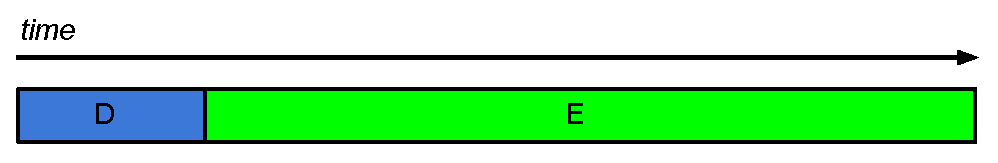
\includegraphics[width=12cm,keepaspectratio]{baseline_scenario_timeline-cropped}
	\caption{Baseline scenarios: a single deliberation phase followed by a single  execution phase.}
	\label{fig:baseline-timeline}
	\end{subfigure}

	\begin{subfigure}[b]{\textwidth}
	\centering
	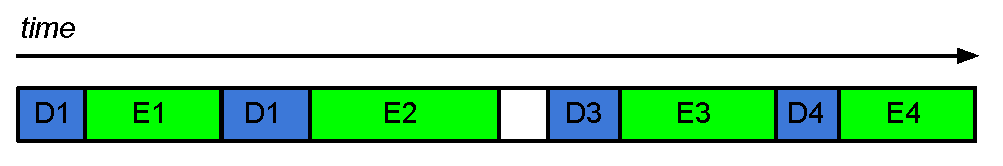
\includegraphics[width=12cm,keepaspectratio]{dynamic_scenario_timeline-cropped}
	\caption{Dynamic scenarios: multiple deliberation and execution phases.}
	\label{fig:dynamic-timeline}
	\end{subfigure}

	\caption{Timelines for baseline and dynamic senarios. \textbf{D$n$} and \textbf{E$n$} indicate deliberation and execution phases, respectively.}
	\label{fig:timelines}
\end{figure}


\begin{figure}[h]
\centering
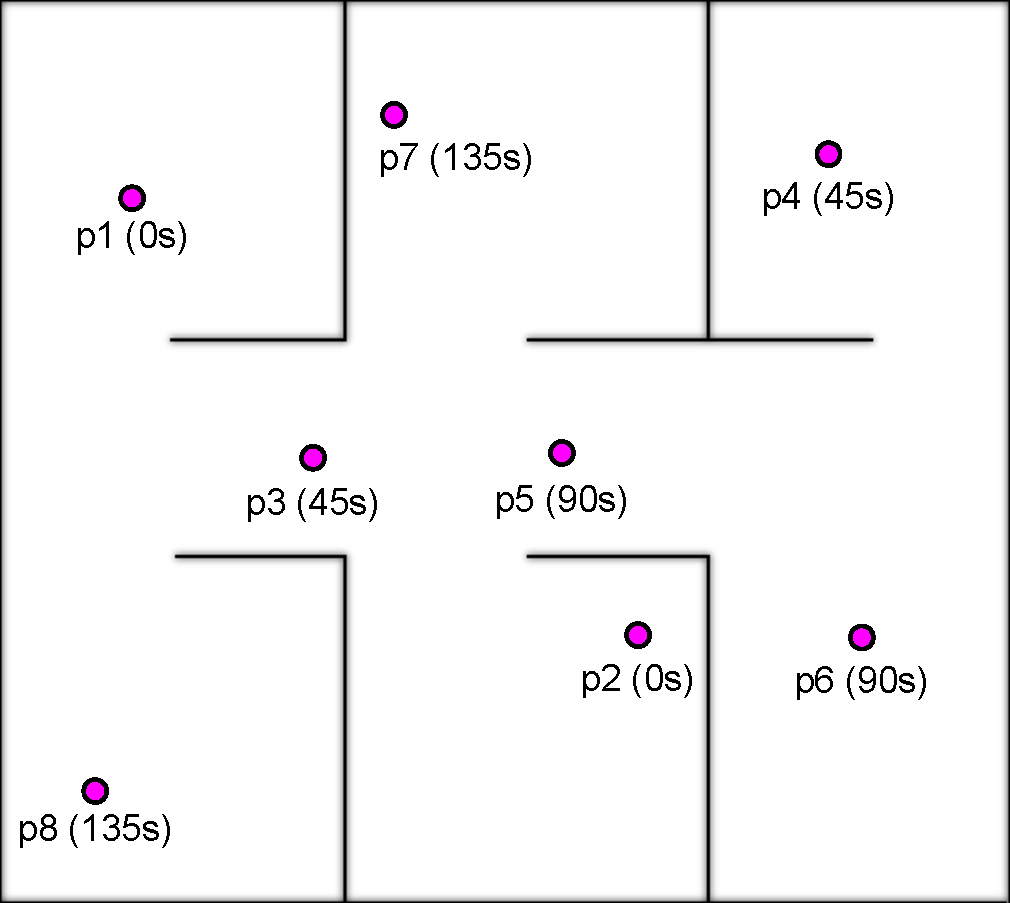
\includegraphics[width=10cm]{TASC_scenario_5}
\caption{Task points for TASC Scenario 5. Each task point \textbf{p$n$} is labelled in the order in which it is introduced ($n$). Each label also indicates how many seconds after the experiment begins that that task is introduced.}
\label{fig:tasc-scenario-5}
\end{figure}


\end{document}
